\documentclass{report}

\usepackage{../../../../../LaTeX/marzstyle}

\runningheads{Programming Language}{Exercise 10}

\setcounter{chapter}{10}

\begin{document}
	\section{Genealogy for covering relations in a family}
	\startsection
	We can define the following rules to define the given relations:
		\begin{minted}{python}
grandfather(X,Y) :- male(X), parent(X,W), parent(W,Y)
grandmother(X,Y) :- female(X), parent(X,W), parent(W,Y)
grandparent(X,Y) :- parent(X,W), parent(W,Y)
grandson(X,Y) :- male(X), parent(W,X), parent(Y,W) 
granddaughter(X,Y) :- female(X), parent(W,X), parent(Y,W) 
grandchild(X,Y) :- parent(W,X), parent(Y,W)
		\end{minted}
	\closesection
	
	\section{Week schedule}
	\startsection
		Using the online prolog compiler https://swish.swi-prolog.org/. We can define the following rules:
		\begin{minted}{python}
day_lecture_compl(monday,english,simple).
day_lecture_compl(tuesday,programming,medium).
day_lecture_compl(tuesday,ai,hard).
day_lecture_compl(wednesday,hacking,hard).
day_lecture_compl(thursday,networking,medium).
day_lecture_compl(friday,pl,easiest).

write_day_schedule(X,Y,Z) :- write(X), write(' - '), write(Y), write(' - '), write(Z), nl.
write_schedule :- forall(day_lecture_compl(X,Y,Z),write_day_schedule(X,Y,Z)).
		\end{minted}
		\begin{tabular}{llc}
			With the command \texttt{?- write\_schedule} we get the following output: & & \multirow{3}{*}{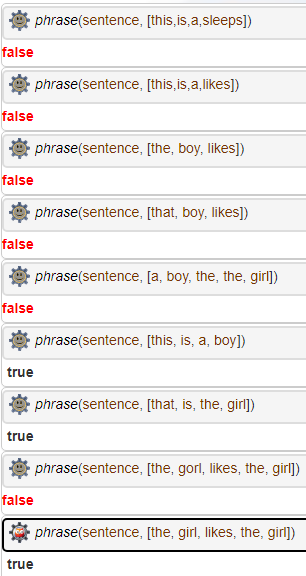
\includegraphics[scale=0.6]{Prolog_Execution.png}} \\
			\\
			\\
			Alternatively we can build it differently by splitting up all the attributes:
		\end{tabular}
		\begin{adjustwidth}{-4em}{}
		\begin{minted}{python}
day(monday). 
day(tuesday). 
day(wednesday). 
day(thursday). 
day(friday).

day_lect(monday,english).
day_lect(tuesday,programming).
day_lect(tuesday,ai).
day_lect(wednesday,hacking).
day_lect(thursday,networking).
day_lect(friday,pl).

lect_compl(english,simple).
lect_compl(programming,medium).
lect_compl(ai,hard).
lect_compl(hacking,hard).
lect_compl(networking,medium).
lect_compl(pl,easiest).

write_schedule :- forall(day(X),write_all(X)).
write_all(X) :- forall(day_lect(X,Y),write_lect_compl(X,Y)).
write_lect_compl(X,Y) :- write(X), write(' - '), write(Y), lect_compl(Y,Z) ,write(' - '), write(Z), nl.
		\end{minted}
		\end{adjustwidth}
		With which the same result will be printed.
	\closesection
\end{document}